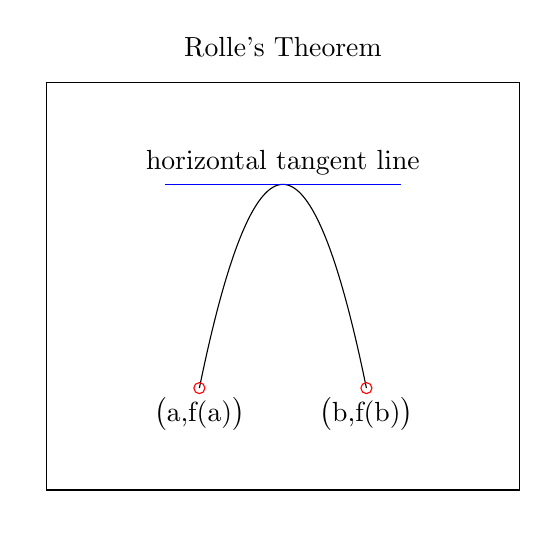
\begin{tikzpicture}
			\begin{axis}[
					scale only axis,
					width  = 6cm,
					xmin   = -1,
					xmax   = 1,
					ymin   = -1,
					ymax   = 1,
					xtick  = \empty,
					ytick  = \empty,
					xlabel = \empty,
					ylabel = \empty,
					title  = Rolle's Theorem,
					smooth,
				]

				\addplot[
					domain  = -1/(2*sqrt(2)):1/(2*sqrt(2)),
					samples = 100,
				]{-8*x^2+0.5};

				% Mark beginning and end
				\addplot [
					only marks,
					color = red,
					mark  = o,
				] coordinates {(-1/(2*sqrt(2)),-0.5) (1/(2*sqrt(2)), -0.5)};

				\addplot [
					color  =blue,
					domain = -0.5:0.5,
				] {0.5};

				% Labels
				\node[above] at (0, 0.5) {horizontal tangent line};
				\node[below] at (-0.3536,-0.5) {\big(a,f(a)\big)};
				\node[below] at (0.3536,-0.5) {\big(b,f(b)\big)};
			\end{axis}
		\end{tikzpicture}
